\documentclass{article}
\usepackage{spalign}
\usepackage{graphicx}
\usepackage{amsmath}
\usepackage{amsfonts}
\usepackage{xcolor}

\title{Introduction to Limits \\ Notes}
\author{John Guzauckas}
\date{\today}

\begin{document}
\maketitle

\section{Objectives}
At the end of this sequence, and after some practice, you should be able to:
\begin{itemize}
    \item Use a calculator to determine right and left hand limits.
    \item Identify right and left hand limits based on graphs.
    \item Determine if a limit exists based on values of right and left hand limits.
    \item Understand that the limit does not depend on the value of a function at the point of interest.
\end{itemize}

\pagebreak
\section{Moving Closer and Closer}
Calculus is all about functions.
\\You probably know that a function $f$ takes an input $x$ and gives an output $f(x)$, which we could write as
$x \mapsto f(x)$.
\\But in calculus, we aren't concerned with just a single input and it's output, we want to consider
a whole range of inputs. We want to know what happens as the input moves/varies.
\\An example: As $x$ moves closer to $1$ from the left: $x \rightarrow 1^{-}$
\begin{center}
    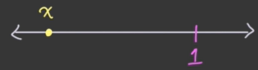
\includegraphics[scale = 1]{Images/MovingCloser1.png}
    \\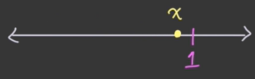
\includegraphics[scale = 1.01]{Images/MovingCloser2.png}        
\end{center}
It is important to note that when we say $x$ moves closer to $1$, we do not mean that $x$ will ever
equal $1$, we are only concerned with values of $x$ that are near $1$.
\\In a function $f$, we know that as we change our input $x$, our output $f(x)$ is going to change as well.
\\With limits, we ask the question, does the output $f(x)$ move close to something as the input $x$
moves close to something?
\\For our example, lets take the function $\frac{\sqrt{3 - 5x + x^{2} + x^{3}}}{x - 1}$.
\\To do this, we could take values for $x$ that are getting closer to $1$ from the left to use as
inputs for $f$.
\\There are an infinite amount of values we could choose for $x$, but we will start with 4 simpler values.
\begin{center}
    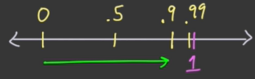
\includegraphics[scale = 1]{Images/MovingCloser3.png}\\
    \begin{tabular} { c|c }
        $x$ & $f(x)$\\
        \cline{1-2} 
        $0$ & $f(0) \approx -1.73$\\
        $0.5$ & $f(0.5) \approx -1.87$\\
        $0.9$ & $f(0.9) \approx -1.97$\\
        $0.99$ & $f(0.99) \approx -1.997$
    \end{tabular}
\end{center}
Reading the values in this table, we can see that as $x$ approaches $1$ from the left, $f(x)$ approaches $-2$.
\\Now we can try to find what $f$ approaches as $x$ approaches $1$ from the right side.
\begin{center}
    \begin{tabular} { c|c }
        $x$ & $f(x)$\\
        \cline{1-2}
        $2$ & $f(2) \approx 2.23$\\
        $1.5$ & $f(1.5) \approx 2.12$\\
        $1.1$ & $f(1.1) \approx 2.02$\\
        $1.01$ & $f(1.01) \approx 2.003$
    \end{tabular}
\end{center}
This time, reading the values in the table, we can see that as $x$ approaches $1$ from the right, $f(x)$
approaches $2$.
\\That means that in this example, the direction we were approaching from with $x$ affected where
$f(x)$ was approaching.

\section{One-Sided Limits}
From the last section, we know that given the function $f(x) = \frac{\sqrt{3 - 5x + x^{2} + x^{3}}}{x - 1}$,
\begin{itemize}
    \item As $x \rightarrow 1^{-}$, $f(x) \rightarrow -2$
    \item As $x \rightarrow 1^{+}$, $f(x) \rightarrow 2$
\end{itemize}
We can plot the points we had in the tables from the last section on the coordinate plane to get a
better picture of what is happening with our function:
\begin{center}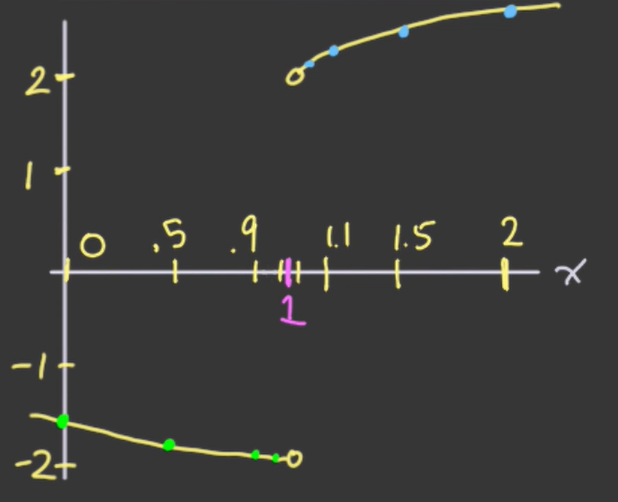
\includegraphics[scale = 0.5]{Images/OneSided1.png}\end{center}
We call this phenomena where a function approaches a value a \textbf{limit}
\\We could rephrase our earlier statements to use our new vocabulary and some new notation:
\begin{itemize}
    \item The limit of $f(x)$ as $x \rightarrow 1^{-}$ is $-2
        \Longrightarrow\underset{x \rightarrow 1^{-}}{\lim} f(x) = -2$
    \item The limit of $f(x)$ as $x \rightarrow 1^{+}$ is $2
        \Longrightarrow\underset{x \rightarrow 1^{+}}{\lim} f(x) = 2$
\end{itemize}
We call the limit as $x$ approaches a value from the left the \textbf{left-hand limit} and the limit
as $x$ approaches a value from the right the \textbf{right-hand limit}.

\section{Definitions of Right-Hand \\and Left-Hand Limits}
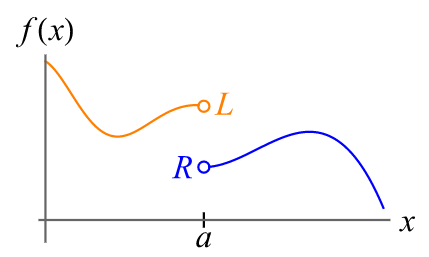
\includegraphics[scale = 1]{Images/RightLeft1.png}\\
Suppose $f(x)$ gets really close to $R$ for values of $x$ that get really close to (but are not equal to)
$a$ from the right. Then we say $R$ is the \textbf{right-hand limit} of the function $f(x)$ as $x$
approaches $a$ from the right. We can write this two different ways:
\[f(x) \rightarrow R \text{ as } x \rightarrow a^{+}\]
\[\underset{x \rightarrow a^{+}}{\lim} f(x) = R\]
If $f(x)$ gets really close to $L$ for values of $x$ that get really close to (but are not equal to) $a$
from the left, we say that $L$ is the \textbf{left-hand limit} of the function $f(x)$ as $x$ approaches
$a$ from the left. We can also write this two different ways:
\[f(x) \rightarrow L \text{ as } x \rightarrow a^{-}\]
\[\underset{x \rightarrow a^{-}}{\lim} f(x) = L\]
Let's explore the right and left-hand limits of a few more functions.

\begin{enumerate}
    \item In this problem, we'll examine the function $g(x) = \frac{x}{\tan(2x)}$ as $x \rightarrow 0^{\pm}$.

Here is a table of values of $g(x)$ as $x$ approaches $0$ from the right:
\begin{center}
    \begin{tabular} { c|c }
        $x$ & $g(x)$\\
        \cline{1-2}
        $1.0$ & $-0.458$\\
        $0.5$ & $0.321$\\
        $0.1$ & $0.493$\\
        $0.05$ & $0.498$\\
        $0.01$ & $0.4999$
    \end{tabular}
\end{center}

These data suggest that $\underset{x \rightarrow 0^{+}}{\lim} g(x) = 0.5$.

Find the left-hand limit:
    \begin{enumerate}
        \item As $x \rightarrow 0^{-}$, $g(x)$ gets closer and closer to a particular number $L$
            $\left(g(x) \rightarrow L\right)$
        \item As $x \rightarrow 0^{-}$, $g(x)$ gets bigger and bigger without bound
            $\left(g(x) \rightarrow +\infty\right)$
        \item As $x \rightarrow 0^{-}$, $g(x)$ gets bigger and bigger in the negative direction without bound
            $\left(g(x) \rightarrow -\infty\right)$
        \item As $x \rightarrow 0^{-}$, $g(x)$ approaches neither a finite number $L$, nor $+\infty$, or $-\infty$.
    \end{enumerate}
\begin{center}
    \begin{tabular} { c|c }
        $x$ & $g(x)$\\
        \cline{1-2}
        $-1.0$ & $-0.457$\\
        $-0.5$ & $0.321$\\
        $-0.1$ & $0.493$\\
        $-0.05$ & $0.498$\\
        $-0.01$ & $0.4999$
    \end{tabular}
\end{center}
The values follow the same trend as the right-hand limit, so $\underset{x \rightarrow 0^{-}}{\lim} g(x) = 0.5$.
This means that (a) is the correct answer, as it is getting closer and closer to a particular number $L$.

\item In this problem, we'll examine the function $h(x) = \frac{|x| + \sin(x)}{x^{2}}$ as $x \rightarrow 0^{\pm}$.

Here is a table of values of $h(x)$ for values of $x$ that are close to zero on the left:
\begin{center}
    \begin{tabular} { c|c }
        $x$ & $h(x)$\\
        \cline{1-2}
        $-1.0$ & $0.159$\\
        $-0.5$ & $0.082$\\
        $-0.1$ & $0.017$\\
        $-0.05$ & $0.002$\\
        $-0.01$ & $0.0002$
    \end{tabular}
\end{center}
These data suggest that $\underset{x \rightarrow 0^{-}}{\lim} h(x) = 0$

Find the right-hand limit:
\begin{enumerate}
    \item As $x \rightarrow 0^{-}$, $h(x)$ gets closer and closer to a particular number $L$
        $\left(h(x) \rightarrow L\right)$
    \item As $x \rightarrow 0^{-}$, $h(x)$ gets bigger and bigger without bound
        $\left(h(x) \rightarrow +\infty\right)$
    \item As $x \rightarrow 0^{-}$, $h(x)$ gets bigger and bigger in the negative direction without bound
        $\left(h(x) \rightarrow -\infty\right)$
    \item As $x \rightarrow 0^{-}$, $h(x)$ approaches neither a finite number $L$, nor $+\infty$, or $-\infty$.
\end{enumerate}
\begin{center}
\begin{tabular} { c|c }
    $x$ & $h(x)$\\
    \cline{1-2}
    $1.0$ & $1.841$\\
    $0.5$ & $3.918$\\
    $0.1$ & $19.983$\\
    $0.05$ & $39.992$\\
    $0.01$ & $199.998$\\
    $0.001$ & $1999.999$
\end{tabular}
\end{center}
The values continue to scale upwards, so $h(x) \rightarrow +\infty$.
This means that (b) is the correct answer, as it is getting bigger and bigger without bound.

\item In this problem, we'll examine the function $j(x) = \sin(\frac{13}{x})$, as $x$ approaches $0$ from
the right. Use a calculator to figure out what $\underset{x \rightarrow 0^{+}}{\lim} j(x)$ might be:
    \begin{enumerate}
        \item As $x \rightarrow 0^{+}$, $j(x)$ gets closer and closer to a particular number $L$
            $\left(j(x) \rightarrow L\right)$
        \item As $x \rightarrow 0^{-}$, $j(x)$ gets bigger and bigger without bound
            $\left(j(x) \rightarrow +\infty\right)$
        \item As $x \rightarrow 0^{-}$, $j(x)$ gets bigger and bigger in the negative direction without bound
            $\left(j(x) \rightarrow -\infty\right)$
        \item As $x \rightarrow 0^{-}$, $j(x)$ approaches neither a finite number $L$, nor $+\infty$, or $-\infty$.
    \end{enumerate}
    \begin{center}
        \begin{tabular} { c|c }
            $x$ & $j(x)$\\
            \cline{1-2}
            $1.0$ & $0.420$\\
            $0.5$ & $0.763$\\
            $0.1$ & $-0.930$\\
            $0.05$ & $0.683$\\
            $0.01$ & $-0.581$\\
            $0.001$ & $0.089$
        \end{tabular}
        \end{center}
This data does not have a clear trend, as it keeps bouncing around values. This must mean that (d) is the
correct answer, as $j(x)$ does not approach a finite number $L$, $+\infty$, or $-\infty$.
\end{enumerate}

\pagebreak
\section{Possible Limit Behaviors}
There are many possible behaviors of limits.

\begin{itemize}
    \item The right-hand and left-hand limits may both exist and be equal.
    \begin{center}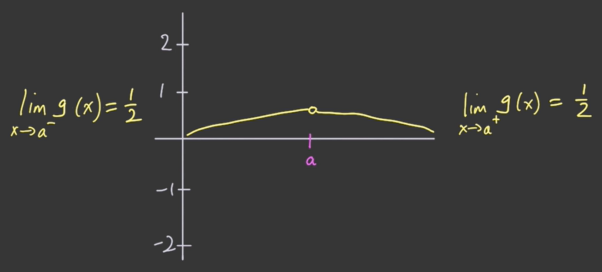
\includegraphics[scale = 0.5]{Images/PossibleBehavior1.png}\end{center}
    \item The right-hand and left-hand limits may both exist, but may fail to be equal.
    \begin{center}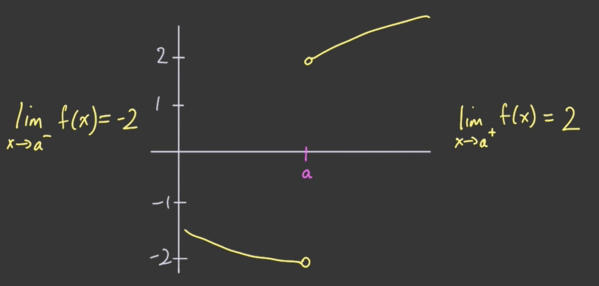
\includegraphics[scale = 0.5]{Images/PossibleBehavior2.png}\end{center}
    \item A right- and/or left-hand limit could fail to exist due to blowing up to $\pm\infty$.
    (Example: Consider the function $\frac{1}{x}$ near $x = 0$.) In this case, we either say the
    limit blows up to infinity, or that the limit does not exist because $\infty$ is not a real number!
    \begin{center}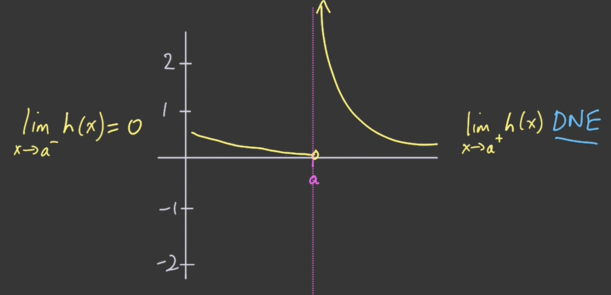
\includegraphics[scale = 0.5]{Images/PossibleBehavior3.png}\end{center}
    \item A right- and/or left-hand limit could fail to exist because it oscillates beteen many values
    and never settles down. In this case, we say the limit does not exist.
    \begin{center}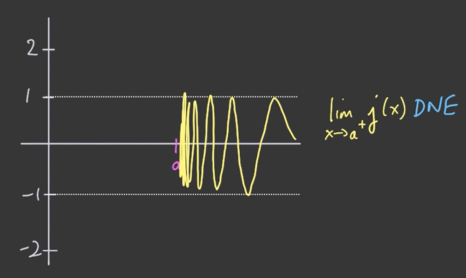
\includegraphics[scale = 0.5]{Images/PossibleBehavior4.png}\end{center}
\end{itemize}

\section{Sample Limit Questions}
\begin{enumerate}
\item Suppose $\underset{x \rightarrow a^{+}}{\lim} f(x)$ exists and equals $R$. Must
    $\underset{x \rightarrow a^{-}}{\lim} f(x)$ exist?

No, $\underset{x \rightarrow a^{-}}{\lim} f(x)$ does not have to exist, as right- and left-hand limits
do not have to be equal, and one could not exist while the other does.

\item Suppose that $\underset{x \rightarrow a^{+}}{\lim} f(x) = R$ and
    $\underset{x \rightarrow a^{-}}{\lim} f(x) = L$. Must $R = L$?

No, the right- and left-hand limits do not have to be the same value even if they both exist.

\item Suppose that $\underset{x \rightarrow a^{+}}{\lim} f(x)$ is some number $R$. Must $f(a) = R$?

No, the limit never checks the actual value of $f(a)$, so the limit can tend towards a value
even if the function has a hole/removable point there.

\item Suppose that $f(a) = K$. Must $\underset{x \rightarrow a^{+}}{\lim} f(x) = K$?

No, the point $(a, K)$ could be a removable point from the function, which the limit would ignore.
\end{enumerate}

\end{document}